% Independently authored V06 fragment. Completed TRAIN findings only.
% Root owns integration and replacement of clearly marked pending results.
\section{Experiments}
\label{sec:experiments}

We separate input representability, actual ranking fit and scheduling
performance. The first two assess the proposed learning mechanism; the third
requires independent deployment evidence. All synthesis conditions use the
same typed library and classical repair kernel. Observed shared-search gains
are therefore not attributed to LLM guidance.

\subsection{Decision Evidence and Authoring Design}
The discovery frame contains 120 unit-weight states: 24 source-induced public
graphs and 96 synthetic contact endpoints forming 48 aligned intervention
pairs. Graphs have at most 32 vertices. Public source clusters are partitioned
within a previously exposed corpus; contact states follow the single-capacity
model in Section~\ref{sec:problem}, with TRAIN ground gap $0\!\to\!1$.
Queries are fixed before certification, retaining all sampling shortfalls.
Across 1,503 endpoint comparisons, 594 preferences are strict, 909 are exact
ties and none remain unknown; 90 strict comparisons have identical base-nine
vectors. Among 630 paired queries, 12 reverse and 123 preserve a strict
preference, 294 tie on both sides, and 201 have one tied endpoint. These
alias-enriched, controlled observations establish information conflicts,
not their incidence in natural satellite operations.

An initial cold-authoring study produced nine of twelve requested eligible
joint selections and identical TRAIN quality across assessed candidates;
we subsequently registered a separate warm-repair study conditional on its
highest-fit ineligible seed and a concrete quotient cycle. This provenance
limits the later comparison to targeted repair of that shared seed.
Witness (W) receives certified relations and concrete equality joins;
relations (R) receives the same relations without joins; objective (O)
receives common quality feedback without those relations. Five fixed blocks
contain eight positions per arm. The first four whole transport-complete
blocks define the preregistered matched cohort; the fifth remains reported.
Slots and requested settings match, whereas actual authoring compute does
not. All 120 positions are valid and finite and return feasible incumbents
on every TRAIN state, giving 14,400 completed assignments.

\subsection{What Witness Feedback Repairs}
Table~\ref{tab:v06-authoring} shows the framework's observed advantage:
the matched information-gate yield is 26/32 for W and 19/32 for R, a
21.875-point difference. Block counts are W/R $7/4,8/4,3/3,8/8$; two favor
W and two tie. The fifth block favors R ($2/5$), reducing the all-block
difference to ten points. Figure~\ref{fig:v06-yield} retains every original
position. These descriptive findings concern conditional interface repair,
not general model efficacy or fully consistent ranking programs.

\begin{table}[t]
\centering
\fontsize{9}{10.4}\selectfont
\setlength{\tabcolsep}{3pt}
\caption{R2 information repair, scalar fit and cost are distinct. Gate entries
are eligible/original positions; raw and joint $m$ are matched-cohort means
out of 594 strict requirements. Work is mean charged feature-plus-repair
operations of joint selections. All present candidates have the same
$q=2693/4480$; O has no joint selection. Bold marks observed column bests.}
\label{tab:v06-authoring}
\begin{tabular}{lrrrrr}
\toprule
Arm & All five & Matched four & Raw $m$ & Joint $m$ & Work\\
\midrule
\textbf{W} & \textbf{28/40} & \textbf{26/32} & 547.91 & 574.00 & 8,441\\
R & 24/40 & 19/32 & \textbf{574.81} & \textbf{579.75} & \textbf{7,850}\\
O & 0/40 & 0/32 & 552.94 & --- & ---\\
\bottomrule
\end{tabular}
\end{table}

\begin{figure}[t]
\centering
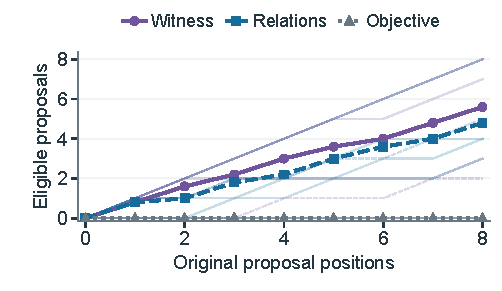
\includegraphics[width=\columnwidth]{figures/refinement_yield_v06.pdf}
\caption{Eligible proposals by original position in all five warm-repair
blocks. Thin curves show individual banks, with the retained fifth dashed;
thick curves average all five. Positions are fixed proposal slots, not
successive learning iterations.}
\label{fig:v06-yield}
\end{figure}

Gate success does not imply scalar consistency. No candidate satisfies all
594 inequalities. Matched raw W fit is lower than R's, retaining the W slot
with only 312 fitted labels; all-five raw means are 553.55, 575.75 and
548.95 for W/R/O. Joint-selected W/R means are 574.00/579.75, while their
base-alias fit is 84.50/83.75 out of 90. W therefore does not dominate R in
rule fit or selected work. Every candidate's exact macro quality is
$2693/4480$, or 60.112\% of total input reward, not an optimum-normalized
score. There is no TRAIN scheduling-quality advantage. Mean author-session
wall times in matched W/R/O are 638.4/700.2/421.6 seconds; equal slot budgets
do not establish equal compute.

Four genuine W joint selections are frozen for deployment. Twelve matched
quality-only selections remain separate nonguarded comparators; their gate
success counts are 3/4 W, 2/4 R and 0/4 O. Comparing W joint against R/O
quality-only therefore compares complete pipelines, including selection,
rather than isolating witness feedback.

\subsection{Complete Quotient Checking and Feature Cost}
The optional catalogue study uses all 53 canonical feature expressions from
the valid cold-authoring bank, the same 594 strict requirements, and capacity
$K=6$. This catalogue is adaptively discovered on TRAIN. Its 4/8/16-expression
prefixes retain an inseparable concrete cycle; none yields an acyclic repair
(Table~\ref{tab:v06-catalogue}). The full catalogue resolves the quotient with
four features at exact minimum additive cost 1,371,468. A separately verified
nonnegative weighting of necessary cuts proves the matching lower bound.

\begin{table}[t]
\centering
\fontsize{9}{10.4}\selectfont
\setlength{\tabcolsep}{4pt}
\caption{All fixed-catalogue outcomes. Rechecks count master trials after
the initial base quotient. Costs of unresolved cyclic subsets are not
reported as repair optima. The minimum concerns standalone operation cost
on this finite catalogue and evidence, not runtime or scalar fit.}
\label{tab:v06-catalogue}
\begin{tabular}{rlrrr}
\toprule
$|\mathcal F|$ & Outcome & Additions & Minimum cost & Rechecks\\
\midrule
4 & Unresolved cycle & --- & --- & 4\\
8 & Unresolved cycle & --- & --- & 7\\
16 & Unresolved cycle & --- & --- & 7\\
53 & \textbf{Acyclic} & 4 & \textbf{1,371,468} & 9\\
\bottomrule
\end{tabular}
\end{table}

Seven self-loop cuts precede two directed-cycle cuts. Eliminating every
self-loop still leaves a cycle; splitting that witness exposes another,
requiring the ninth full-inventory recheck. Figure~\ref{fig:v06-catalogue}
shows this progression and cost composition. Neighborhood packing, root
deletion, continuation-edge count and continuation clique cover contribute
2.18\%, 10.73\%, 28.78\% and 58.31\% of the minimum. The last primitive
dominates this additive proxy. Greedy tie orders are retained, so invariance
under identifier renaming is not assumed. The result validates scoped
representation repair; it does not supply a fitted scalar or a runtime optimum.

\begin{figure*}[t]
\centering
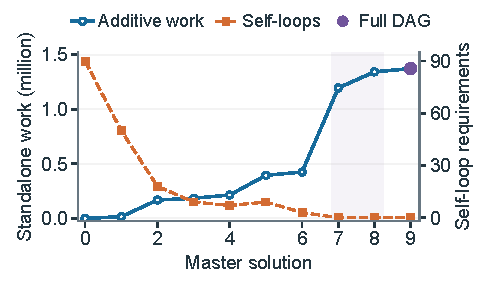
\includegraphics[width=.48\textwidth]{figures/refinement_cost_curve_v06.pdf}\hfill
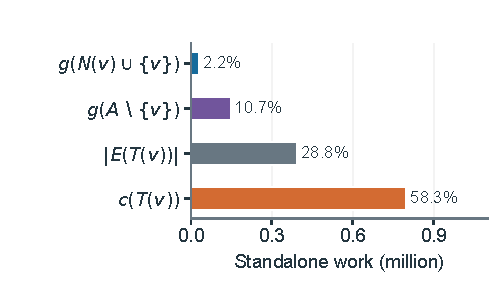
\includegraphics[width=.48\textwidth]{figures/refinement_feature_work_v06.pdf}
\caption{Fixed-catalogue repair on TRAIN. Left: additive cost and full
quotient obstructions across master trials; intermediate cyclic subsets are
not successful repairs. Right: standalone work of the four features attaining
the certified catalogue minimum. Feature work here excludes shared-DAG savings
and remains distinct from complete-policy measured cost.}
\label{fig:v06-catalogue}
\end{figure*}

\subsection{Published Solvers and Shared-Component Calibration}
Table~\ref{tab:v06-native} reports the complete assessed native method set
on 25 WDP and three UAI Segmentation TRAIN sources. Native stochastic methods
use three fixed seeds; deterministic methods and Degree use one. Across
0.1/1/5-second nominal targets, 633 of 1,008 assignments return checked
feasible incumbents. The other 375 are explicit encoding limitations;
unsupported objectives remain absent, not zero. Original weights are retained
through recorded exact transformations. WDP and Segmentation rewards are
reported separately.

\begin{table*}[t]
\centering
\fontsize{9}{10.4}\selectfont
\setlength{\tabcolsep}{5pt}
\caption{Completed TRAIN native calibration at the common one-second nominal
target: raw objective mean (higher is better), feasible/assigned coverage and
median wrapper wall seconds. Bold denotes best observed reward and lowest
wall time among valid outputs within each family. $\dagger$ denotes input
rejection latency, with no solver reward. These are calibration results,
not comparisons against the proposed frozen programs.}
\label{tab:v06-native}
\begin{tabular}{lrrr rrr}
\toprule
& \multicolumn{3}{c}{WDP} & \multicolumn{3}{c}{UAI Segmentation}\\
Method & Raw reward & Coverage & Wall & Raw reward & Coverage & Wall\\
\midrule
CHILS~\cite{grossmann2025chils} & \textbf{84,224,796.39} & 75/75 & 1.509 & \textbf{1,670.450} & 9/9 & 1.014\\
CHILS ILS~\cite{grossmann2025chils} & 84,221,656.72 & 75/75 & 1.516 & \textbf{1,670.450} & 9/9 & 1.019\\
M2WIS~\cite{grossmann2024mmwis} & --- & 0/75 & $0.003^\dagger$ & \textbf{1,670.450} & 9/9 & 0.075\\
Struction~\cite{gellner2021struction} & --- & 0/25 & $0.004^\dagger$ & \textbf{1,670.450} & 3/3 & 0.024\\
WeightedBR~\cite{lamm2019weighted} & --- & 0/25 & $0.003^\dagger$ & \textbf{1,670.450} & 3/3 & \textbf{0.021}\\
Shared Degree repair & 48,279,098.24 & 25/25 & \textbf{1.000} & 1,663.217 & 3/3 & 0.347\\
\bottomrule
\end{tabular}
\end{table*}

Measured costs differ from internal targets: WDP CHILS median wrapper times
are 0.598/1.509/5.521 seconds at targets 0.1/1/5. Encoding, startup and
validation prevent interpreting these as matched hard deadlines. A separate
32-source component calibration returns feasible incumbents for all 960
assignments. Warm Degree repair improves its matched half-target CHILS seed
in only 4/288 cases; against full-target CHILS it wins/ties/loses in
2/222/64. Stronger common components therefore do not yet demonstrate a
framework quality advantage, and these calibration outcomes did not enter
R2 authoring or selection.

\subsection{Frozen Evaluation: Pending Result Inputs}
The separate evaluation plan retains 72 withheld mechanism states and five
prescribed identifier renamings. Its performance inventory has 302 contexts:
216 fresh weighted contact endpoints, 25 WDP, three Segmentation, ten
numerically compatible Grids and 48 exploratory C3 contexts. Two common
initialization tracks, three targets and 23 policy identities, including four
EoH-style typed comparison runs~\cite{liu2024eoh}, define 52,548 assignments.
C3 reuse is reported separately; source-specific numerical compatibility,
null identities, measured initialization/repair cost and coverage remain visible.
Frozen selection uses no evaluation outcome.

\textit{[DRAFT RESULT INPUT: insert independently verified EoH authoring and
TRAIN-selection outcomes; do not treat the current W/R/O ablation as an EoH
reproduction.]}

\textit{[DRAFT RESULT INPUT: insert withheld reversal/preservation and
renaming results, then complete raw-quality/actual-cost/coverage comparisons
with every published solver and all frozen policies. No such result is
available in this fragment.]}

\textit{[DRAFT RESULT INPUT: insert the separately released TRAIN patch-ranking
bridge with core versus full-strict pair strata and separate local/full target
scopes. Inclusion-preference fit must not be described as pivot-efficiency
certification.]}
